\chapter{class notes}
    \section{Coulomb's Law}
    \begin{eqboxed}{eq:CoulombsLaw}{Coulomb's Law}
    {Gives a force along the line of two charges. \\ If \(q_1\) and \(q_2\) have the same sign (i.e. charge) then the force must be repulsive. But if they have the \textit{same} sign, then it must be attractive.\\ 
    Because of Newton's second law, \(F_{12} = -F_{21}\)}
    \vec{F_{12}} =k\frac{q_1q_2}{r_{12}^2}\hat{r_{12}} 
    \end{eqboxed}

\begin{center}
  % \boxed{\vec{F_{12}} =k\frac{q_1q_2}{r_{12}^2}\hat{r_{12}}}
  \begin{tikzpicture}[>=Stealth, thick]
    % --- Positions ---
    \coordinate (q1) at (0,0);
    \coordinate (q2) at (5,0);
  
    % --- Dotted separation line ---
    \draw[densely dotted] (q1) -- (q2);
  
    % --- Charges as filled circles ---
    \fill[blue!70!black] (q1) circle (5pt);

  
    % --- Labels for charges ---
    \node[above left=-1pt and -2pt] at (q1) {$q_1$};
    \node[above left=-1pt and -2pt] at (q2) {$q_2$};
    \node[] at (q1) {$+$};

  
    % --- Force arrow from q2 to the right ---
    \draw[white, very thick, ->] (q2) -- ++(2.2,0)
      node[midway, above] {$\vec{F}_{12}$};

    \fill[blue!70!black] (q2) circle (5pt);
    \node[] at (q2) {$+$};

    % --- r_12 arrow below ---
    \draw[->] ($(q1)+(0,-0.9)$) -- ($(q2)+(0,-0.9)$)
      node[midway, below] {$\vec{r}_{12}$};
  \end{tikzpicture}

    \begin{tikzpicture}[>=Stealth, thick]
    % --- Positions ---
    \coordinate (q1) at (0,0);
    \coordinate (q2) at (5,0);
  
    % --- Dotted separation line ---
    \draw[densely dotted] (q1) -- (q2);
  
    % --- Charges as filled circles ---
    \fill[red!70!black] (q1) circle (5pt);

  
    % --- Labels for charges ---
    \node[above left=-1pt and -2pt] at (q1) {$q_1$};
    \node[above left=-1pt and -2pt] at (q2) {$q_2$};
    \node[] at (q1) {$-$};

  
    % --- Force arrow from q2 to the right ---
    \draw[white, very thick, ->] (q2) -- ++(-2.2,0)
      node[midway, above] {$\vec{F}_{12}$};

    \fill[blue!70!black] (q2) circle (5pt);
    \node[] at (q2) {$+$};

    % --- r_12 arrow below ---
    \draw[->] ($(q1)+(0,-0.9)$) -- ($(q2)+(0,-0.9)$)
      node[midway, below] {$\vec{r}_{12}$};
  \end{tikzpicture}

  \pagebreak

  \boxed{F_{1,net} = F_{21} + F_{31}}

  \begin{tikzpicture}[>=Stealth, thick]
    % --- Positions ---
    \coordinate (q1) at (0,0);
    \coordinate (q2) at (5,0);
    \coordinate (q3) at (0,-5);
  
    % --- Dotted separation line ---
    \draw[densely dotted] (q1) -- (q2);
    \draw[densely dotted] (q1) -- (q3);
  
    % --- Charges as filled circles ---


    \draw[white, very thick, ->] (q1) -- ++(2.2,0)
      node[midway, above] {$\vec{F}_{21}$};

    \draw[white, very thick, ->] (q1) -- ++(0,-2.2)
      node[midway, left] {$\vec{F}_{31}$};

    \draw[white, very thick, ->] (q1) -- ++(2,-2)
      node[midway, left] {$\vec{F}_{net}$};

    \fill[blue!70!black] (q1) circle (5pt);

    % --- Labels for charges ---
    \node[above left] at (q1) {$q_1$};
    \node[below right] at (q2) {$q_2$};
    \node[below right] at (q3) {$q_3$};
    \node[] at (q1) {$-$};

  
    % --- Force arrow from q2 to the right ---
    % \draw[white, very thick, ->] (q2) -- ++(-2.2,0)
    %   node[midway, above] {$\vec{F}_{12}$};

    %       % --- Force arrow from q2 to the right ---
    % \draw[white, very thick, ->] (q3) -- ++(0,2.2)
    %   node[midway, right] {$\vec{F}_{13}$};


    \fill[red!70!black] (q2) circle (5pt);
    \node[] at (q2) {$+$};

    \fill[red!70!black] (q3) circle (5pt);
    \node[] at (q3) {$+$};


    % % --- r_12 arrow below ---
    % \draw[->] ($(q1)+(0,-0.9)$) -- ($(q2)+(0,-0.9)$)
    %   node[midway, below] {$\vec{r}_{12}$};
  \end{tikzpicture}

\end{center}

\begin{eqboxed}{eq:SuperpostionPrinciple}{Superpostion Principle}
{}
F_{net} = \sum_i \vec{F_i}
\end{eqboxed}
\begin{constboxed}{const:e}{Electron Charge}
{}
e = -1.6 \times 10^{-19} C
\end{constboxed}

\begin{constboxed}{const:k}{k}
{}
k = 9 \times 10^9 \frac{NM^2}{C^2}
\end{constboxed}


\pagebreak
\subsection{Examples}
\hrule
\vspace{.5cm}


\begin{example}

\begin{center} 
  \boxed{F_{3,net}= ???}\vspace{.5cm}
      \begin{tikzpicture}[>=Stealth, thick]
      % --- Positions ---
      \coordinate (q1) at (-5,0);
      \coordinate (q2) at (0,0);
      \coordinate (q3) at (5,0);
    
      % --- Dotted separation line ---
      \draw[densely dotted] (q1) -- (q2);
      \draw[densely dotted] (q1) -- (q3);
    
      % --- Charges as filled circles ---
      
      \draw[white, very thick, <->] ($(q1) +(0,-1.5)$) -- ($(q2) +(-.2,-1.5)$)
        node[midway, below] {$1m$};

      \draw[white, very thick, <->] ($(q2) +(+.2,-1.5)$) -- ($(q3) +(0,-1.5)$)
        node[midway, below] {$1m$};

  
      \draw[white, very thick, ->] ($(q3) +(0,-.4)$) -- ++(1.2,0)
        node[midway, below] {$\vec{F}_{13}$};
  
  
      \draw[white, very thick, ->] ($(q3) +(0,-.5)$) -- ++(-2.2,0)
        node[midway, below] {$\vec{F}_{23}$};
  
      \fill[blue!70!black] (q1) circle (5pt);
      \node[] at (q1) {$-$};

      % --- Labels for charges ---
      \node[below right] at (q1) {$q_1$};
      \node[below right] at (q2) {$q_2$};
      \node[below right] at (q3) {$q_3$};

      \node[above] at (q1) {$q_1 = 2  \mu C$};
      \node[above] at (q2) {$q_2 = -1 \mu C$};
      \node[above] at (q3) {$q_3 = 4  \mu C$};
  
    
      % --- Force arrow from q2 to the right ---
      % \draw[white, very thick, ->] (q2) -- ++(-2.2,0)
      %   node[midway, above] {$\vec{F}_{12}$};
  
      %       % --- Force arrow from q2 to the right ---
      % \draw[white, very thick, ->] (q3) -- ++(0,2.2)
      %   node[midway, right] {$\vec{F}_{13}$};
  
  
      \fill[red!70!black] (q2) circle (5pt);
      \node[] at (q2) {$+$};
  
      \fill[blue!70!black] (q3) circle (5pt);
      \node[] at (q3) {$-$};
  
  
      % % --- r_12 arrow below ---
      % \draw[->] ($(q1)+(0,-0.9)$) -- ($(q2)+(0,-0.9)$)
      %   node[midway, below] {$\vec{r}_{12}$};
      \end{tikzpicture}
\end{center}

\hrule
\vspace{.5cm}
Using Coulomb's Law\ref{eq:CoulombsLaw}\dots
\[
\vec{F_{3,net}} = \vec{F_{31}} + \vec{F_{32}} \]
\[\vec{F_{31}} = k \frac{q_3q_1}{r_{31}^2} \hat{r_{32}}\]
\[\vec{F_{32}} = k \frac{q_3q_2}{r_{32}^2} \hat{r_{32}}\]
\[k = 9 \times 10^9 \frac{NM^2}{C^2},  \qquad q_1 = 2\mu C, \qquad q_2 = -1 \mu C, \qquad q_3 = 4\mu C \]
\[\vec{F_{31}} = \SI{1.800e-02}{\N}, \quad \vec{F_{32}} = \SI{-3.600e-02}{\N}\]
\[\boxed{\vec{F}_{3, net} =  \SI{-1.800e-02}{\N}}\]
\end{example}


\pagebreak
\section{Electric flux and Field Lines·}
\hrule
\vspace{.5cm}

\subsection{Field Lines}
\begin{list}{-}{}
\item Measure of electric field lines over an area
\end{list}

\begin{eqboxed}{eq:ElectricField}{Electric Field}
{Measure of the energy in an electric field at a point}
E = k \frac{q}{r^2}
\end{eqboxed}

\begin{eqboxed}{eq:fieldlineDensity}{Density of Field Lines}
{used when plotting}
D = \frac{N}{4 \pi r^2}
\end{eqboxed}

\begin{eqboxed}{eq:numberOfLines}{Number of Graphed Field Lines }
{}
N \equiv \frac{q}{\epsilon_0}, \quad E = \frac{N}{A}
\end{eqboxed}
\subsection{Flux}
Number of field lines passing through a surface 
\[\Phi \propto N\]

For a point charge aligned at the center at a sphere it can just be defined as 
\[\Phi \equiv EA \]

To calculate total over surface \dots
\[\Phi \equiv \int_{s} \vec{E} \dot d\vec{A}\]

\pagebreak
\section{5: potential energy}
\hrule
\vspace{.5cm}

\begin{eqboxed}{eq:GausssLaw}{Guass's Law}
{}
\int E dS = \frac{Q_{enclosed}}{\epsilon_0}
\end{eqboxed}

\begin{eqboxed}{eq:Change_in_Potential}{Change in potential in const E field}
{}
\Delta U = q \vec{E} \ell
\end{eqboxed}

\begin{eqboxed}{eq:Change_in_pot_in_non_static}{Change in potential in non static field}
{}
\Delta U = Q\int_a^b \vec{E} dr 
\end{eqboxed}

\pagebreak
\setcounter{section}{6}
\section{Conductors and Capacitance}
\hrule
\vspace{.5cm}

\subsection{Conductors}
\begin{list}{-}{}
\item Every point in a conductor is at equipotential, this is because the electric field at any point is zero.
\item Contuining with Gausses law, no matter the location of a charge contained \textit{inside} a shell (but not overlapping the shell itself), the outside of the shell will have the same charge distribution, however the inside may not.
\item When looking at the inverse, (a particle placed \textit{outside} of a conductor), we find that the charges move to the surface to cancel out the exerted field, meaning that the inside of the object will have a net charge of 0. 
\item Importantly, this still applies when a cavity is made \textit{within the conductor}
\item This allows for the shielding of an object if it is placed within a conductor \footnote{Think Faraday cage (maybe)}
\end{list}

\pagebreak
\begin{example}
  \begin{center}

    \textbf{Equipotential difference in two Spheres} 
    \vspace{.1cm}
    \hrule
    \vspace{.25cm}
      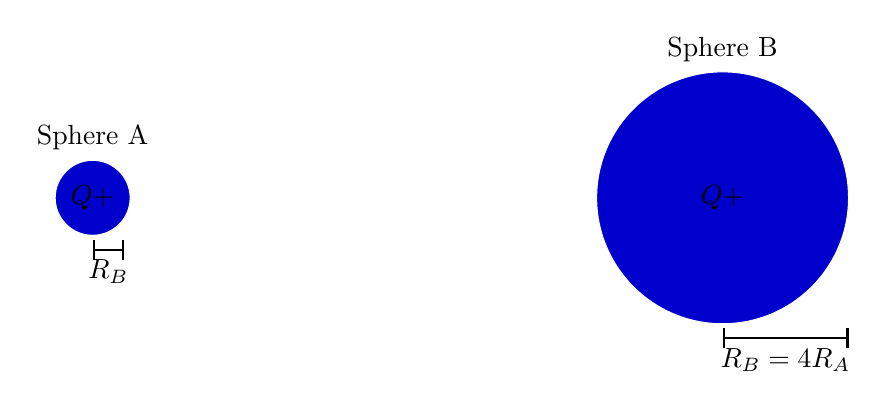
\begin{tikzpicture}
          \node[draw=white, fill=blue!80!black, circle, minimum size=.8cm, label={above:Sphere A}] (A) at (-4,0) {$Q+$}; 

          \node[draw=white, fill=blue!80!black, circle, minimum size=3.2cm,label={above:Sphere B}] (B) at (4,0) {$Q+$}; 

          \draw[thick, |-|] ([yshift=-5pt]B.south) -- ++(1.6cm,0) 
          node[midway, below] {$R_B = 4R_A$};

          \draw[thick, |-|] ([yshift=-5pt]A.south) -- ++(0.4cm,0) 
          node[midway, below] {$R_B$};

      \end{tikzpicture}
      \[
      V_A = - \int_{\infty}^{R_A} \vec{E}_A \cdot \vec{dl},
      \qquad 
      V_B = - \int_{\infty}^{R_B} \vec{E}_B \cdot \vec{dl}
      \]
      Given a point charge \dots
      \[
      \vec{E} = k\frac{Q}{r^2} 
      \rightarrow 
      -\int_{\infty}^{r} k \frac{Q}{r^2} = k \frac{Q}{r}
      \rightarrow 
      \]
      For a point charge\dots
      \[V = k \frac{Q}{r}\]
      \[
      V_A = k \frac{Q}{R_A},
      \qquad
      V_B = k \frac{Q}{4 R_B}
      \]
      \[
      4 \times V_A = V_B 
      \]
      Once connected, become a single conductor which wishes to reach equipotential. To find final charges \dots
      \[
      V_A = V_B 
      \rightrightarrows
      k \frac{Q_A}{R_A} = k \frac{Q_B}{R_B}
      \] 
      \[
      \cancel{k} \frac{Q_A}{R_A} = \cancel{k} \frac{Q_B}{4 R_A}
      \]
      \[
      4Q_A = Q_B
      \]


  \end{center}
\end{example}

\pagebreak
\subsection{Capacitance}
\begin{eqboxed}{eq:Capacitance}{Capacitance}
{Units of Farads, or Coulombs per volt}
C \equiv \frac{Q}{\Delta V}
\end{eqboxed}
\begin{list}{-}{}
\item Measure of field between to oppositely charged objects
\item Ex. A plate of Q and -Q placed a distance d away from one another 
\item Stores the energy \textit{in} the magnetic field induced between said objects
\end{list}

\begin{example}
  \begin{center}
    \textbf{Capacitance between two plates}
    \vspace{.1cm}
    \hrule
    \vspace{.25cm}
    \begin{tikzpicture}[>=Stealth]

    % --- 1. Top Plate (+Q) ---
    \draw[fill=blue] (-2, 0.8) rectangle (2, 1.0);
    \node[above=5pt] at (0, 1.0) {\large $+Q$};

    % --- 2. Bottom Plate (-Q) ---
    \draw[fill=red] (-2, -1.0) rectangle (2, -0.8);
    \node[below=5pt] at (0, -1.0) {\large $-Q$};

    % --- 3. Distance Label 'd' ---
    % Drawing a vertical line between the inner edges of the plates
    \draw[thick, |-|] (-2.2, 0.8) -- (-2.2, -0.8) 
        node[midway, left=2pt] {$d$};

    \draw[thick, |-|] (-2, 2) -- (2, 2) 
        node[midway, above=2pt] {$L$};

    \draw[thick, |-|] (2.2, 0.8) -- (2.2, -0.8) 
        node[midway, right=2pt] {$V$};


    \draw[thick, ->] (0, 0.8) -- (0, -0.8);
    \draw[thick, ->] (1, 0.8) -- (1, -0.8);
    \draw[thick, ->] (-1, 0.8) -- (-1, -0.8);
        node[midway, right=10pt] {$\vec{E}$};
    
    \node[] at (-.2, -2.5) {$\boxed{d << L}$};
      

      
    \end{tikzpicture}

    To calculate E field between plates \dots
    \[
    E_{bot} = \frac{1}{2} \frac{\sigma}{\epsilon_0},
    \quad 
    E_{top} = \frac{1}{2} \frac{\sigma}{\epsilon_0}
    \]
    \[
    \sigma = \frac{Q}{A}
    \]
    \[
    E_{bot} = \frac{1}{2} \frac{Q}{\epsilon_0 A },
    \quad 
    E_{top} = \frac{1}{2} \frac{Q}{\epsilon_0 A}
    \]
    Since field lines are the same direction\dots
    \[
    E_{tot} = \frac{Q}{\epsilon_0 A}
    \]
    
    To find capacitance\dots
    \[
    C \equiv \frac{Q}{\Delta V}
    \]
    \[
    \left|\Delta V\right| = \int_{bot}^{top} \vec{E} \cdot dl 
    \rightrightarrows
    \Delta V = \frac{Q}{\epsilon_0 A} \int_{bot}^{top} dl 
    \] 
    \[
    \Delta V = \frac{Q}{\epsilon_0 A} d
    \]
    \[
    C = \frac{\epsilon_0 A}{d}
    \]

  \end{center}
\end{example}
\begin{eqboxed}{eq:capacitance_for_parrel_plates}{Capacitance for Parrel Plates}
{}
C = \frac{\epsilon_0 A}{d}
\end{eqboxed}
\begin{example}
  \begin{center}
    \textbf{Parallel Plate Capacitor}
    \vspace{.1cm}
    \hrule
    \vspace{.25cm}
    \begin{tikzpicture}[>=Stealth]

    % --- 1. Top Plate (+Q) ---
    \draw[fill=blue] (-2, 0.8) rectangle (2, 1.0);
    \node[above=5pt] at (0, 1.0) {\large $+Q$};

    % --- 2. Bottom Plate (-Q) ---
    \draw[fill=red] (-2, -1.0) rectangle (2, -0.8);
    \node[below=5pt] at (0, -1.0) {\large $-Q$};

    % --- 3. Distance Label 'd' ---
    % Drawing a vertical line between the inner edges of the plates

    \draw[thick, |-|] (2.2, 0.8) -- (2.2, -0.8) 
        node[midway, right=2pt] {$V$};


    \draw[thick, ->] (1, 0.8) -- (1, -0.8);
    \draw[thick, ->] (-1, 0.8) -- (-1, -0.8);
    \node[right=5pt] at (.9, 0) {$\vec{E}$};


    \draw[thick, dashed, ->] (0, -0.8) -- (0, .3);
    \fill[blue] (0,0) circle (2.5pt);
    \node[right=.5pt] at (0, -.25) {${dq}$};
    \end{tikzpicture}

    To calculate the work needed to move a particle from the bottom plate to the top plate 
    \[dW = dq E d\]
    Since we know that the energy from the electric field is equal to \(\frac{V}{d}\)\dots
    \[
    dW = dq \frac{V}{\cancel{d}} \cancel{d}
    \]
    \[
    dU = V dq
    \]
    This holds true for \textit{any system}. Note that dU is \textit{not} constant because for each particle moved, it becomes requires more work for the next. 
    
    To calculate potential of a capacitor\dots

    \[
    U = \int_{0}^{Q} V dq 
    \rightrightarrows
    U = \int_{0}^{Q} \frac{q}{c} dq
    \]

    Thus \dots
    \[
    U = \frac{1}{2} \frac{Q^2}{C}
    \]
  \end{center}
\end{example}
\pagebreak
\begin{eqboxed}{eq:Capacitor_potential}{Potential of a Capacitor}
{}
U = \frac{1}{2} \frac{Q^2}{C} \quad 
U = \frac{1}{2} CV^2 \quad 
U = \frac{1}{2} QV
\end{eqboxed}

\begin{eqboxed}{eq:capacitor_energy_density}{Energy density of a capacitor}
{}
u = \frac{1}{2} \epsilon_0 E^2
\end{eqboxed}
